% Springer LNCS format. Build:  tectonic paper.tex   (or pdflatex with llncs.cls)
% Every number is taken from docs/PAPER_RESULTS.md; chart data comes from data/paper_eval/.
\documentclass[runningheads]{llncs}

\usepackage[T1]{fontenc}
\usepackage{graphicx}
\usepackage{amsmath}
\usepackage{booktabs}
\usepackage{array}
\usepackage{xcolor}
\usepackage{tikz}
\usetikzlibrary{positioning,arrows.meta,calc}
\usepackage{pgfplots}
\pgfplotsset{compat=1.17}
\usepackage[hidelinks]{hyperref}

\definecolor{ink}{HTML}{1F4E79}
\definecolor{inklight}{HTML}{9DB9D5}
\definecolor{warm}{HTML}{C0504D}
\definecolor{sand}{HTML}{D9A441}
\definecolor{sage}{HTML}{6A9A6E}
\definecolor{grey}{HTML}{8C8C8C}

% shared chart style
\pgfplotsset{
  value labels/.style={nodes near coords={\pgfmathprintnumber[fixed,fixed zerofill,precision=1]{\pgfplotspointmeta}}},
  small chart/.style={
    width=\linewidth, height=4.1cm,
    tick label style={font=\scriptsize}, label style={font=\scriptsize},
    title style={font=\scriptsize\bfseries, yshift=-1mm},
    legend style={font=\tiny, draw=none, fill=none},
    axis lines*=left, ymajorgrids, grid style={grey!25}},
}

\begin{document}

\title{Plan, Gate, Learn: A Verified Multi-Agent Orchestrator for Natural-Language Cloud Data Pipelines}
\titlerunning{Plan, Gate, Learn}

% TODO(authors): replace the placeholders below before submission.
\author{Manvith M. Nayak\inst{1} \and Co-Author Name\inst{1}}
\authorrunning{M. M. Nayak et al.}
\institute{Department / Institution, City, Country\\
\email{manvithnayak8704@gmail.com}}

\maketitle

\begin{abstract}
Describing a data pipeline takes one sentence; building it on a cloud platform takes an
afternoon of containers, copy activities, Spark code and compute settings. We built an
orchestrator in which nine agents turn a CSV file and a plain-English request into a
running Azure Data Factory and Databricks pipeline, and we measured where each agent earns
its place. A 7B model fine-tuned with QLoRA understands 96\% of unseen requests, against
33\% before tuning, but only a deterministic repair step makes its plans runnable (33\% to
100\%); a 120B cloud model given the same rules is correct on 53\%. A structural gate stops
every one of 1{,}400 injected plan faults before the cloud, two thirds of which would
otherwise have produced wrong data without any error. On live Azure runs, a fix to the
learning loop cut duration-estimate error from 53.6\% to 14.4\%, and learned corrections cut
cost-estimate error by 41--47\%. We also report what went wrong: a learned abort rule that
is right only 54\% of the time, and a silent data corruption that only output checks caught.

\keywords{LLM agents \and data pipelines \and fine-tuning \and verification \and self-adaptive systems}
\end{abstract}

% ===========================================================================
\section{Introduction}

Suppose an analyst wants the average order value per region, but only for orders with more
than five items. On Azure this means creating storage containers, a linked service, datasets
and a Data Factory copy pipeline, writing and debugging a Databricks notebook of 100--200 lines,
and picking throughput units, workers and shuffle partitions that fit the subscription. Mistakes
show up late. A filter on a misspelled column compiles without complaint and fails inside Spark,
after the cluster has already been paid for.

Language models can write such a configuration, and that is where the trouble starts. A plan that
is almost right does not run. A plan that runs may quietly answer a different question. And
nothing in the model knows what a run will cost or how long it will take. Our orchestrator
treats all three as separate problems, gives each decision to exactly one agent, and puts a
deterministic check behind every learned component.

The paper makes four contributions: (i) a planner that combines a small fine-tuned model,
deterministic repair and a single self-verification step, and beats a 120B cloud model on the
same contract (Sect.~\ref{sec:planner}); (ii) layered gates, evaluated with 1{,}400 injected
faults, that keep wrong plans out of the cloud (Sect.~\ref{sec:gates}); (iii) a closed learning
loop with evidence gates and automatic rollback, evaluated live and in simulation
(Sect.~\ref{sec:learning}); and (iv) a live Azure evaluation in which every output was checked
against a reference, including the failures (Sect.~\ref{sec:live},~\ref{sec:lessons}).

% ===========================================================================
\section{Related Work}

Agents that reason and act~\cite{react}, reflect~\cite{reflexion} or refine their own
output~\cite{selfrefine}, and frameworks that split work across agents~\cite{autogen,metagpt},
make LLMs more capable on multi-step tasks. Without outside feedback, though, models rarely fix
their own reasoning~\cite{selfcorrect}, which is why our planner only re-plans on feedback from
checks it cannot argue with. Text-to-SQL work~\cite{spider,rajkumar} shows strong but brittle
generation of single queries; a pipeline plan also fixes storage, stage wiring and resources, so
small mistakes stop it from running at all. LoRA~\cite{lora} and QLoRA~\cite{qlora} make it cheap to
specialise a base model such as Qwen2.5~\cite{qwen25}. Learned tuning of data
systems~\cite{ottertune} and the MAPE-K loop of autonomic computing~\cite{autonomic} shaped our
predictors and learning loop; we add evidence gating and rollback, and show where rollback itself
goes wrong.

% ===========================================================================
\section{System}
\label{sec:design}

\begin{figure}[t]
\centering
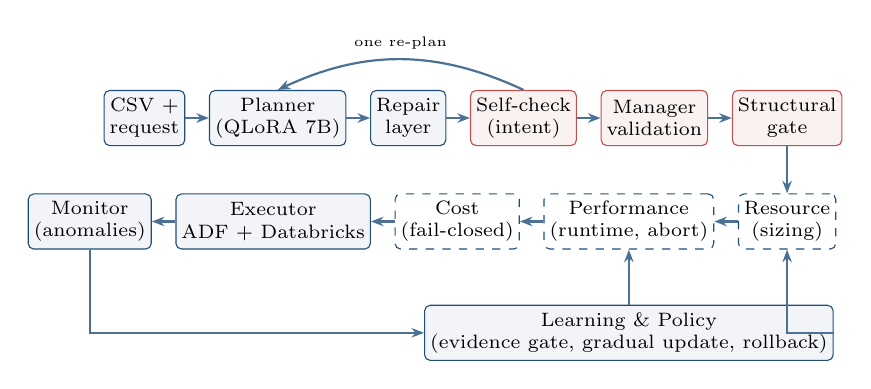
\begin{tikzpicture}[
  font=\scriptsize,
  box/.style={draw=ink, rounded corners=2pt, align=center, minimum height=7mm, inner sep=2pt, fill=ink!6},
  gate/.style={draw=warm, rounded corners=2pt, align=center, minimum height=7mm, inner sep=2pt, fill=warm!8},
  ml/.style={draw=ink, dashed, rounded corners=2pt, align=center, minimum height=7mm, inner sep=2pt},
  arr/.style={-{Stealth[length=1.6mm]}, draw=ink!80, thick}]
\node[box] (in) {CSV +\\request};
\node[box, right=3mm of in] (pl) {Planner\\(QLoRA 7B)};
\node[box, right=3mm of pl] (rep) {Repair\\layer};
\node[gate, right=3mm of rep] (sc) {Self-check\\(intent)};
\node[gate, right=3mm of sc] (val) {Manager\\validation};
\node[gate, right=3mm of val] (gt) {Structural\\gate};
\node[ml, below=6mm of gt] (res) {Resource\\(sizing)};
\node[ml, left=3mm of res] (perf) {Performance\\(runtime, abort)};
\node[ml, left=3mm of perf] (cost) {Cost\\(fail-closed)};
\node[box, left=3mm of cost] (ex) {Executor\\ADF + Databricks};
\node[box, left=3mm of ex] (mon) {Monitor\\(anomalies)};
\node[box, below=7mm of perf] (learn) {Learning \& Policy\\(evidence gate, gradual update, rollback)};
\draw[arr] (in) -- (pl); \draw[arr] (pl) -- (rep); \draw[arr] (rep) -- (sc);
\draw[arr] (sc) -- (val); \draw[arr] (val) -- (gt); \draw[arr] (gt) -- (res);
\draw[arr] (res) -- (perf); \draw[arr] (perf) -- (cost); \draw[arr] (cost) -- (ex);
\draw[arr] (ex) -- (mon);
\draw[arr] (sc.north) to[bend right=25] node[above, font=\tiny]{one re-plan} (pl.north);
\draw[arr] (mon.south) |- (learn.west);
\draw[arr] (learn.east) -| (res.south);
\draw[arr] (learn.north) -- (perf.south);
\end{tikzpicture}
\caption{Life of a run. Solid boxes are deterministic, dashed boxes are learned, and red
boxes can stop a run before any cloud spend.}
\label{fig:arch}
\end{figure}

Figure~\ref{fig:arch} shows the path of a request. The Planner designs the pipeline, the
Resource Agent picks compute settings within the subscription's limits, the Performance Agent
forecasts runtime and may abort a run it expects to fail, the Cost Agent looks for cheaper
settings, and the Executor deploys the copy and runs the notebooks. The Central Manager only
sequences these agents and enforces their verdicts. Each decision has one owner. This rule
came from experience: in an earlier version the runtime model's strongest input (importance
0.91) was the Resource Agent's own runtime guess, so two agents were silently predicting the
same thing. Independent stages run concurrently as \emph{execution groups}, and streaming plans
process only new files on each tick.

\paragraph{Planner.} We generated 5{,}000 training examples (schema, request, plan) across 18
domains and 2--5 stages. An independent validator enforces 19 rules covering structure, value
ranges, one filter grammar and semantic sanity, such as no contradictory filters. Every row
passes. An earlier template-based dataset failed at least one rule in every row
(Fig.~\ref{fig:data}b). We tuned Qwen2.5-7B-Instruct~\cite{qwen25} with QLoRA~\cite{qlora}
(4-bit base, rank 16) on a single Tesla T4 in 4.5 hours, training 0.53\% of the parameters; the
adapter is an 81\,MB file served locally. Each raw plan then goes through a deterministic repair
layer (Azure-safe names, stage wiring, operator types, size-aware caps) and a self-check: the
structural rules plus an intent check by a separate, untuned 7B model. If the check finds a
problem, the planner re-plans once with that problem as feedback.

The intent checker needed help. Given only the request and raw JSON, it invented column names
and flagged correct plans. Once it saw the real columns and a plain-language description of each
stage, and two simple rules discarded complaints about non-existent columns or changes the plan
already made, its accuracy on a fixed test suite rose from 15/18 to 27/27.

\paragraph{Learning loop.} Every five runs, the Learning \& Policy Agent compares predictions with
what actually happened. A correction factor changes only after at least 10 relevant runs, moves
30\% of the way toward the observed ratio, and is reverted if error rises by more than 5\% over the
next five runs. When runtime error passes 20\%, the runtime model is retrained with real runs
blended in and kept only if held-out error does not get worse.

\begin{figure}[t]
\begin{minipage}[t]{0.49\linewidth}
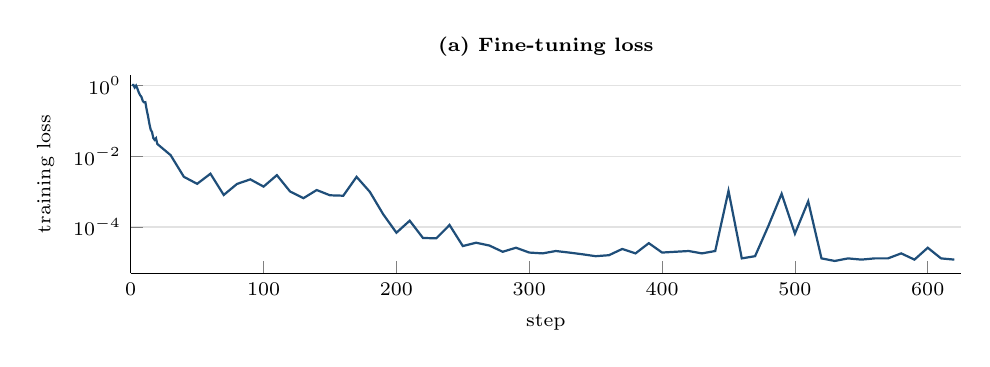
\begin{tikzpicture}
\begin{axis}[small chart, ymode=log, xmin=0, xmax=625, ymin=5e-6, ymax=2,
  title={(a) Fine-tuning loss}, xlabel={step}, ylabel={training loss},
  ytick={1,1e-2,1e-4,1e-6}]
\addplot[ink, thick, mark=none] coordinates {(1,1.02001) (2,1.03301) (3,0.872716) (4,0.985856) (5,0.814936) (6,0.638874) (7,0.533234) (8,0.479058) (9,0.367045) (10,0.334006) (11,0.33672) (12,0.20451) (13,0.136084) (14,0.083906) (15,0.056334) (16,0.048578) (17,0.032692) (18,0.028988) (19,0.032162) (20,0.022178) (30,0.010746) (40,0.002619) (50,0.001661) (60,0.003208) (70,0.000805) (80,0.001649) (90,0.00222) (100,0.001387) (110,0.002919) (120,0.001004) (130,0.000653) (140,0.001108) (150,0.000788) (160,0.000767) (170,0.002615) (180,0.000985) (190,0.000231) (200,6.9e-05) (210,0.000151) (220,4.9e-05) (230,4.8e-05) (240,0.000114) (250,2.9e-05) (260,3.6e-05) (270,3e-05) (280,2e-05) (290,2.6e-05) (300,1.9e-05) (310,1.8e-05) (320,2.1e-05) (330,1.9e-05) (340,1.7e-05) (350,1.5e-05) (360,1.6e-05) (370,2.4e-05) (380,1.8e-05) (390,3.5e-05) (400,1.9e-05) (410,2e-05) (420,2.1e-05) (430,1.8e-05) (440,2.1e-05) (450,0.001052) (460,1.3e-05) (470,1.5e-05) (480,0.000107) (490,0.000869) (500,6.5e-05) (510,0.000532) (520,1.3e-05) (530,1.1e-05) (540,1.3e-05) (550,1.2e-05) (560,1.3e-05) (570,1.3e-05) (580,1.8e-05) (590,1.2e-05) (600,2.6e-05) (610,1.3e-05) (620,1.2e-05)};
\end{axis}
\end{tikzpicture}
\end{minipage}\hfill
\begin{minipage}[t]{0.49\linewidth}
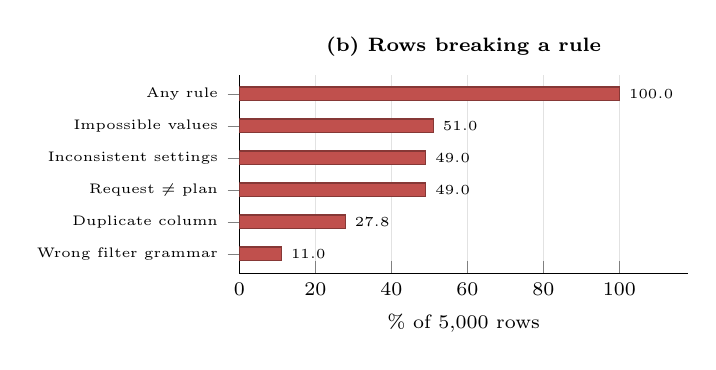
\begin{tikzpicture}
\begin{axis}[small chart, xbar, xmin=0, xmax=118, bar width=5pt, width=0.6\linewidth,
  title={(b) Rows breaking a rule},
  xlabel={\% of 5{,}000 rows},
  symbolic y coords={Wrong filter grammar,Duplicate column,Request $\neq$ plan,Inconsistent settings,Impossible values,Any rule},
  ytick=data, y tick label style={font=\tiny}, ymajorgrids=false, xmajorgrids,
  enlarge y limits=0.12,
  value labels, nodes near coords style={font=\tiny}]
\addplot[fill=warm, draw=warm!70!black] coordinates {(11.0,Wrong filter grammar) (27.8,Duplicate column) (49.0,Request $\neq$ plan) (49.0,Inconsistent settings) (51.0,Impossible values) (100,Any rule)};
\end{axis}
\end{tikzpicture}
\end{minipage}
\caption{(a) Training loss over 625 steps (one epoch, T4): the plan grammar is learned within
about 100 steps, which is why we test on requests phrased unlike the training data.
(b) Share of rows in the earlier template dataset that break each rule; the validated dataset breaks none.}
\label{fig:data}
\end{figure}

% ===========================================================================
\section{Experimental Setup}

\emph{Planner.} We wrote 24 requests over three schemas (sales, zoo animals, IoT sensors), in the
way people actually ask: ``drop the cheap stuff'', ``only EU region rows please'', a misspelled
``filtr rows whre quantiy~>~10'', aggregations and numbered multi-stage requests. A plan is
\emph{executable} if it passes the structural and safety checks and every stage compiles to
PySpark, and \emph{meets intent} if the requested operations appear (patterns fixed in advance).
It is \emph{correct} if both hold. Raw and repaired outputs are scored on the same sample.

\emph{Live runs.} All runs used an Azure for Students subscription (Data Factory copy,
Databricks serverless, Blob storage) through the production API, with seeded CSVs of 1{,}000,
50{,}000 and 400{,}000 rows (0.06--25.5\,MB). We downloaded every output and compared it with a
reference computed locally from the same file. Estimates were logged before each run and only
used earlier runs. Errors are MAPE. Local inference ran on an Apple M5 with 16\,GB.

% ===========================================================================
\section{Results}

\subsection{Each part of the planner does a different job}
\label{sec:planner}

\begin{figure}[t]
\centering
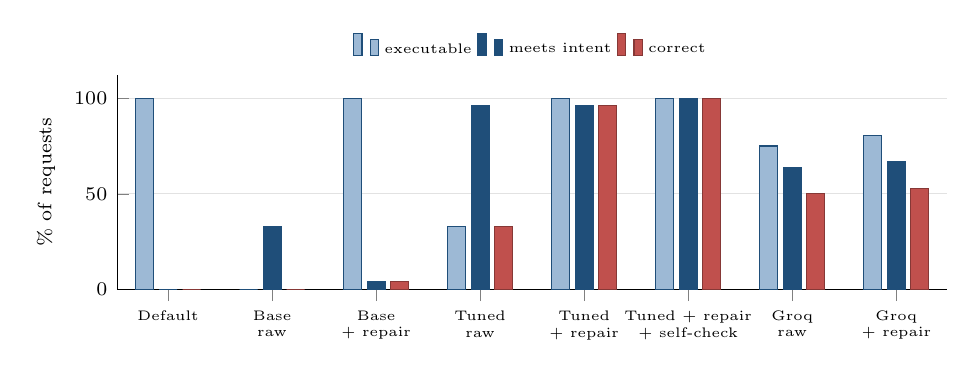
\begin{tikzpicture}
\begin{axis}[small chart, ybar, height=4.3cm, bar width=6.5pt,
  ymin=0, ymax=112, ylabel={\% of requests},
  symbolic x coords={Default,Base raw,Base+repair,Tuned raw,Tuned+repair,+ self-check,Groq raw,Groq+repair},
  xtick=data, x tick label style={font=\tiny, align=center},
  xticklabels={Default,{Base\\raw},{Base\\+ repair},{Tuned\\raw},{Tuned\\+ repair},{Tuned + repair\\+ self-check},{Groq\\raw},{Groq\\+ repair}},
  legend style={at={(0.5,1.03)}, anchor=south, legend columns=3},
  enlarge x limits=0.07]
\addplot[fill=inklight, draw=ink] coordinates {(Default,100) (Base raw,0) (Base+repair,100) (Tuned raw,33) (Tuned+repair,100) (+ self-check,100) (Groq raw,75.0) (Groq+repair,80.6)};
\addplot[fill=ink, draw=ink] coordinates {(Default,0) (Base raw,33) (Base+repair,4) (Tuned raw,96) (Tuned+repair,96) (+ self-check,100) (Groq raw,63.9) (Groq+repair,66.7)};
\addplot[fill=warm, draw=warm!70!black] coordinates {(Default,0) (Base raw,0) (Base+repair,4) (Tuned raw,33) (Tuned+repair,96) (+ self-check,100) (Groq raw,50.0) (Groq+repair,52.8)};
\legend{executable, meets intent, correct}
\end{axis}
\end{tikzpicture}
\caption{Planner ablation on 24 unseen requests. ``Default'' is the deterministic fallback plan;
``Base'' is untuned Qwen2.5-7B; ``Groq'' is gpt-oss-120b given the full rule book (mean of 3
runs, s.d.\ 2--4 points). The self-check bar covers the 12 requests where it was run.}
\label{fig:planner}
\end{figure}

Figure~\ref{fig:planner} shows that no single component is enough. The deterministic default
always runs and never does what was asked. The untuned model understands a third of the requests
but writes plans in the wrong shape, and repair cannot save them: the system falls back to the
default plan in 15 of 24 cases. Fine-tuning lifts intent to 96\%, yet only a third of its raw plans
run. When a request names no containers, the model invents names Azure rejects, or wires a stage to
read and write the same container. Repair fixes all of these without touching intent, and the
self-check catches the one remaining miss, a missing aggregation, on its single re-plan.

The 120B cloud model behaves differently. With the whole rule book in its prompt, 75\% of its raw
plans already run, so repair adds little; it loses on intent. Some of that gap is a matter of style:
it writes filters as \texttt{equals(region,'EU')}, which our patterns do not count, so its numbers are
a lower bound. Even so, the small local model is right far more often, costs nothing per plan and keeps
the data on the machine. The cloud model is about twice as fast (19.7\,s against 41\,s per plan) at
roughly a tenth of a cent.

\subsection{Gates keep wrong plans out of the cloud}
\label{sec:gates}

\begin{figure}[t]
\begin{minipage}[t]{0.49\linewidth}
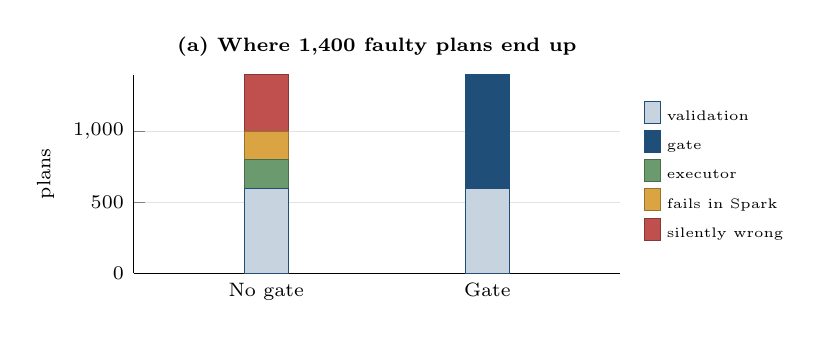
\begin{tikzpicture}
\begin{axis}[small chart, ybar stacked, bar width=16pt, ymin=0, ymax=1400,
  width=0.64\linewidth,
  title={(a) Where 1{,}400 faulty plans end up},
  symbolic x coords={No gate,Gate}, xtick=data,
  enlarge x limits=0.6, ylabel={plans},
  legend style={at={(1.03,0.5)}, anchor=west}, legend cell align=left]
\addplot[fill=ink!25, draw=ink] coordinates {(No gate,600) (Gate,600)};
\addplot[fill=ink, draw=ink] coordinates {(No gate,0) (Gate,800)};
\addplot[fill=sage, draw=sage!70!black] coordinates {(No gate,200) (Gate,0)};
\addplot[fill=sand, draw=sand!70!black] coordinates {(No gate,200) (Gate,0)};
\addplot[fill=warm, draw=warm!70!black] coordinates {(No gate,400) (Gate,0)};
\legend{validation, gate, executor, fails in Spark, silently wrong}
\end{axis}
\end{tikzpicture}
\end{minipage}\hfill
\begin{minipage}[t]{0.49\linewidth}
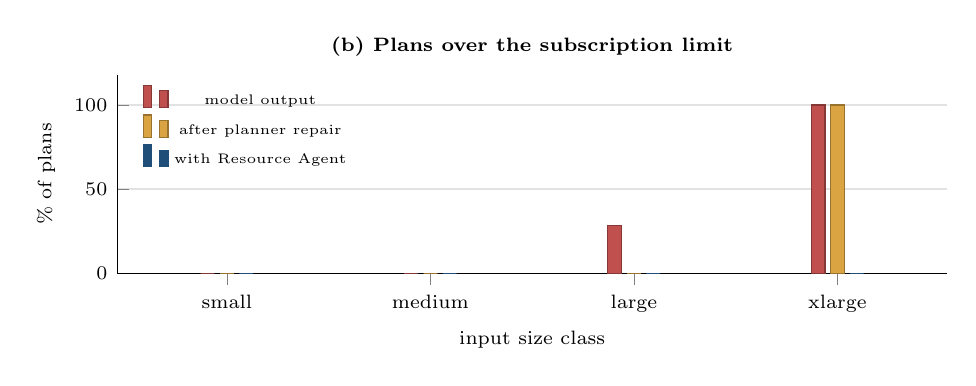
\begin{tikzpicture}
\begin{axis}[small chart, ybar, bar width=5pt, ymin=0, ymax=118,
  title={(b) Plans over the subscription limit},
  symbolic x coords={small,medium,large,xlarge}, xtick=data,
  xlabel={input size class}, ylabel={\% of plans},
  legend style={at={(0.02,0.98)}, anchor=north west}, enlarge x limits=0.18]
\addplot[fill=warm, draw=warm!70!black] coordinates {(small,0) (medium,0) (large,28.4) (xlarge,100)};
\addplot[fill=sand, draw=sand!70!black] coordinates {(small,0) (medium,0) (large,0) (xlarge,100)};
\addplot[fill=ink, draw=ink] coordinates {(small,0) (medium,0) (large,0) (xlarge,0)};
\legend{model output, after planner repair, with Resource Agent}
\end{axis}
\end{tikzpicture}
\end{minipage}
\caption{(a) Seven kinds of fault injected into 200 valid plans each and followed through the real
checks. Without the structural gate, 600 reach Databricks and 400 of those run ``successfully'' with
wrong output. (b) Share of 1{,}000 plans that ask for more compute than the subscription allows.}
\label{fig:gates}
\end{figure}

We took 200 valid plans and broke each one in seven ways, from a filter on a missing column to a code
injection string, then followed every broken plan through the real checks in run order
(Fig.~\ref{fig:gates}a). The Manager's own validation catches malformed plans, and the executor
refuses code it cannot compile. But both are tolerant by design: an unknown stage type is skipped
and an unsupported aggregation such as \texttt{median} is dropped. Without the gate, 43\% of the faulty
plans reach the cloud, and two thirds of those do not even fail. They just produce the wrong numbers.
With the gate, none get through. It takes 0.07\,ms per plan.

Writing this harness also found a bug in the gate itself: type names inside \texttt{cast(x as double)}
were read as columns, so 12.3\% of valid plans were rejected. After a one-line configuration fix,
0 of 5{,}000 are. Compute sizing is a gate of its own (Fig.~\ref{fig:gates}b). Even after the
planner's own size caps, every extra-large plan asks for more copy throughput than the student tier
allows; with the Resource Agent, none do.

\subsection{Live on Azure}
\label{sec:live}

\begin{figure}[t]
\begin{minipage}[t]{0.49\linewidth}
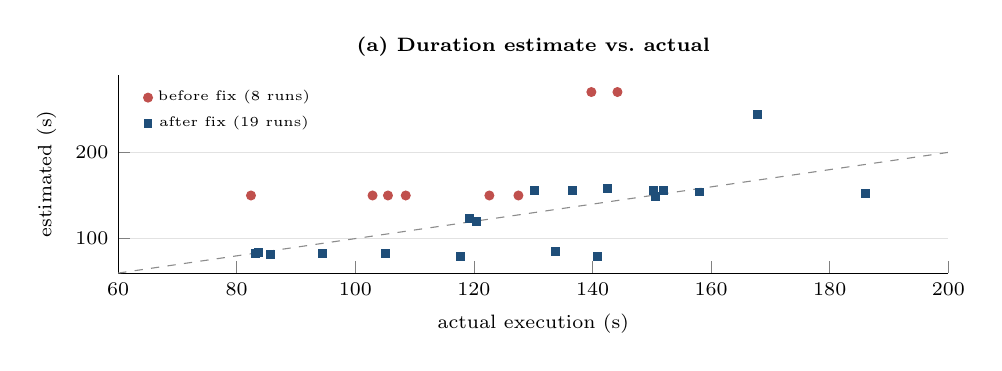
\begin{tikzpicture}
\begin{axis}[small chart, xmin=60, xmax=200, ymin=60, ymax=290,
  title={(a) Duration estimate vs.\ actual},
  xlabel={actual execution (s)}, ylabel={estimated (s)},
  legend style={at={(0.02,0.98)}, anchor=north west, fill=white}]
\addplot[grey, dashed, domain=60:200, samples=2, forget plot] {x};
\addplot[only marks, mark=*, mark size=1.6pt, color=warm] coordinates {(102.9,150) (144.2,270) (108.5,150) (127.5,150) (82.4,150) (139.8,270) (105.5,150) (122.6,150)};
\addplot[only marks, mark=square*, mark size=1.4pt, color=ink] coordinates {(117.8,79) (150.6,149) (140.9,79) (186.0,152) (136.6,156) (83.2,83) (142.5,158) (133.7,85) (167.8,244) (83.6,84) (150.3,156) (105.1,83) (152.0,156) (119.2,123) (94.5,83) (130.2,156) (85.7,82) (158.0,154) (120.4,120)};
\legend{before fix (8 runs), after fix (19 runs)}
\end{axis}
\end{tikzpicture}
\end{minipage}\hfill
\begin{minipage}[t]{0.49\linewidth}
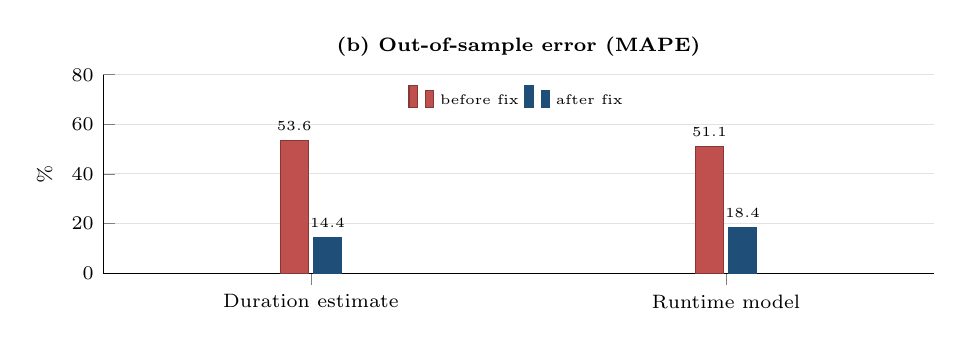
\begin{tikzpicture}
\begin{axis}[small chart, ybar, bar width=10pt, ymin=0, ymax=80,
  title={(b) Out-of-sample error (MAPE)},
  symbolic x coords={Duration estimate,Runtime model}, xtick=data,
  ylabel={\%}, enlarge x limits=0.5,
  nodes near coords, nodes near coords style={font=\tiny},
  legend style={at={(0.5,0.98)}, anchor=north, legend columns=2, fill=white}]
\addplot[fill=warm, draw=warm!70!black] coordinates {(Duration estimate,53.6) (Runtime model,51.1)};
\addplot[fill=ink, draw=ink] coordinates {(Duration estimate,14.4) (Runtime model,18.4)};
\legend{before fix, after fix}
\end{axis}
\end{tikzpicture}
\end{minipage}
\caption{Estimates made before each live run. After removing a cold-start floor that had blocked
duration learning, the points move onto the diagonal. One run delayed 15 minutes inside Databricks is
left out of the ``after'' set; with it, the errors are 18.3\% and 22.0\%.}
\label{fig:fix}
\end{figure}

\paragraph{Prediction.} Looking through the feedback log, we noticed that the Resource Agent's learned
duration correction did nothing: every corrected notebook estimate was pushed back up to a fixed
120\,s cold-start floor. Removing the floor, and learning one ratio per run and per size band, moved the
estimates onto the diagonal (Fig.~\ref{fig:fix}). On a fresh batch of 24 runs, duration error fell from
53.6\% to 14.4\% and runtime-model error from 51.1\% to 18.4\%. The runtime model improved because the
duration estimate is its strongest input. That input is the ``circular'' feature from Sect.~\ref{sec:design},
and we tested dropping it: live error then rose from 36.5\% to 142.1\%. The feature is informative; the
fix is to replace it with the Resource Agent's settings, not to delete it.

\begin{figure}[t]
\begin{minipage}[t]{0.49\linewidth}
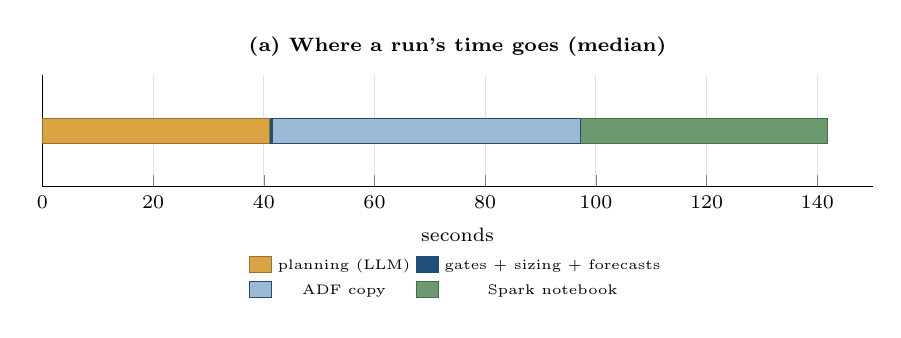
\begin{tikzpicture}
\begin{axis}[small chart, xbar stacked, bar width=9pt, xmin=0, xmax=150,
  title={(a) Where a run's time goes (median)},
  symbolic y coords={run}, ytick=\empty, enlarge y limits=0.6, height=3.0cm,
  xlabel={seconds}, ymajorgrids=false, xmajorgrids,
  legend style={at={(0.5,-0.55)}, anchor=north, legend columns=2}]
\addplot[fill=sand, draw=sand!70!black] coordinates {(41,run)};
\addplot[fill=ink, draw=ink] coordinates {(0.6,run)};
\addplot[fill=inklight, draw=ink] coordinates {(55.6,run)};
\addplot[fill=sage, draw=sage!70!black] coordinates {(44.7,run)};
\legend{planning (LLM), gates + sizing + forecasts, ADF copy, Spark notebook}
\end{axis}
\end{tikzpicture}
\end{minipage}\hfill
\begin{minipage}[t]{0.49\linewidth}
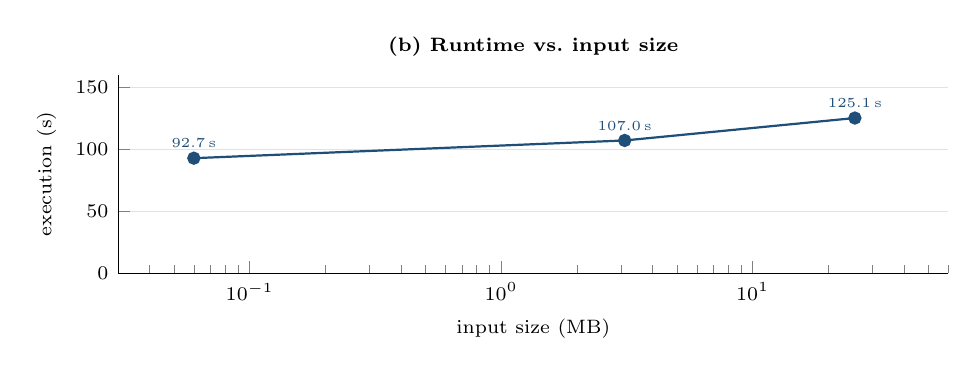
\begin{tikzpicture}
\begin{axis}[small chart, xmode=log, xmin=0.03, xmax=60, ymin=0, ymax=160,
  title={(b) Runtime vs.\ input size},
  xlabel={input size (MB)}, ylabel={execution (s)},
  nodes near coords, point meta=explicit symbolic, nodes near coords style={font=\tiny, anchor=south}]
\addplot[ink, thick, mark=*] coordinates {(0.06,92.7)[92.7\,s] (3.1,107.0)[107.0\,s] (25.5,125.1)[125.1\,s]};
\end{axis}
\end{tikzpicture}
\end{minipage}
\caption{(a) Median time per run over 14 live runs: the system's own decisions take under a second;
almost everything else is Azure start-up. (b) A 418$\times$ larger file takes only 35\% longer.}
\label{fig:time}
\end{figure}

\paragraph{Time.} A request becomes verified output in two to three and a half minutes. Planning takes
29--53\,s, and the run itself a median of 116\,s. Of that, the system's own decisions (validation, gates,
sizing, forecasts, code generation) take less than one second; the rest is Azure copying data and
starting Spark (Fig.~\ref{fig:time}). That is also why runtime barely depends on input size at this
scale. Per pipeline, the system writes 108--195 lines of PySpark and 5--7 Data Factory objects that
someone would otherwise have to write by hand.

\begin{figure}[t]
\begin{minipage}[t]{0.49\linewidth}
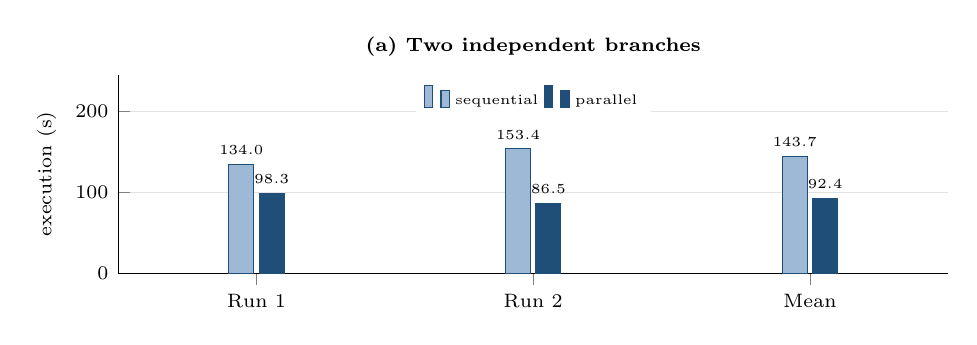
\begin{tikzpicture}
\begin{axis}[small chart, ybar, bar width=9pt, ymin=0, ymax=245,
  title={(a) Two independent branches},
  symbolic x coords={Run 1,Run 2,Mean}, xtick=data, ylabel={execution (s)},
  enlarge x limits=0.25, legend style={at={(0.5,0.98)}, anchor=north, legend columns=2, fill=white},
  value labels, nodes near coords style={font=\tiny}]
\addplot[fill=inklight, draw=ink] coordinates {(Run 1,134.0) (Run 2,153.4) (Mean,143.7)};
\addplot[fill=ink, draw=ink] coordinates {(Run 1,98.3) (Run 2,86.5) (Mean,92.4)};
\legend{sequential, parallel}
\end{axis}
\end{tikzpicture}
\end{minipage}\hfill
\begin{minipage}[t]{0.49\linewidth}
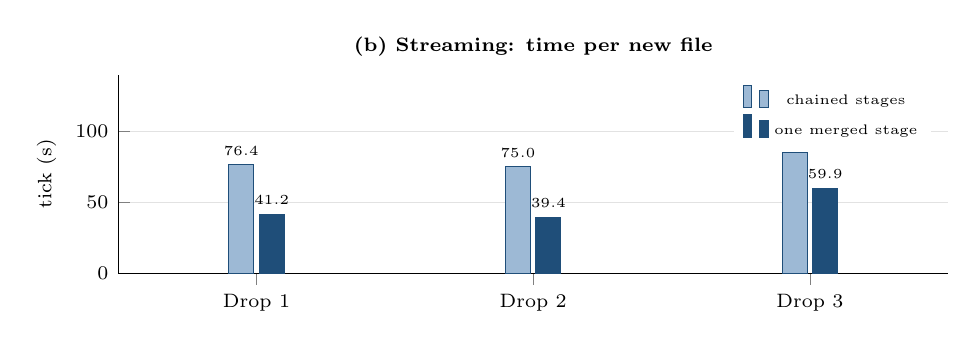
\begin{tikzpicture}
\begin{axis}[small chart, ybar, bar width=9pt, ymin=0, ymax=140,
  title={(b) Streaming: time per new file},
  symbolic x coords={Drop 1,Drop 2,Drop 3}, xtick=data, ylabel={tick (s)},
  enlarge x limits=0.25, legend style={at={(0.98,0.98)}, anchor=north east, fill=white},
  value labels, nodes near coords style={font=\tiny}]
\addplot[fill=inklight, draw=ink] coordinates {(Drop 1,76.4) (Drop 2,75.0) (Drop 3,85.1)};
\addplot[fill=ink, draw=ink] coordinates {(Drop 1,41.2) (Drop 2,39.4) (Drop 3,59.9)};
\legend{chained stages, one merged stage}
\end{axis}
\end{tikzpicture}
\end{minipage}
\caption{(a) Running two independent notebook stages as one execution group saves about one Spark
start-up ($-36\%$). (b) Merging two streaming steps into one stage is 41\% faster per new file, with
identical output (285, 567 and 852 cumulative rows; about 300 expected per drop).}
\label{fig:exec}
\end{figure}

\paragraph{Execution choices.} Because start-up dominates, anything that avoids a second Spark job pays
off (Fig.~\ref{fig:exec}). Running two independent branches together cut 143.7\,s to 92.4\,s. For
streaming, one merged stage handled each new file in 46.8\,s instead of 78.8\,s, and every file was
processed exactly once.

\paragraph{Correct output.} Of the 20 runs in the last batch that completed, 16 produced exactly the
reference result. All four failures came from one plan, which we come back to in
Sect.~\ref{sec:lessons}. Pinning the planner's own settings instead of the Resource Agent's made no
measurable difference on the smaller files; on the 25\,MB file the Resource Agent chose half the copy
throughput and the copy took 81\,s instead of 60\,s. Its value is in staying within limits, not in speed.

\subsection{The learning loop}
\label{sec:learning}

\begin{figure}[t]
\begin{minipage}[t]{0.49\linewidth}
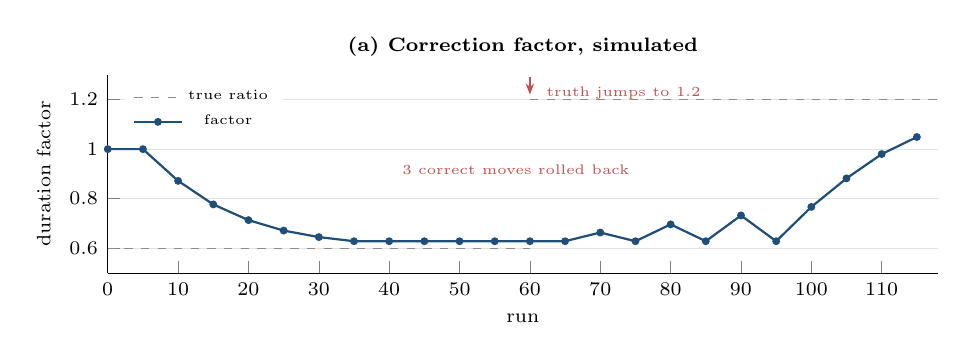
\begin{tikzpicture}
\begin{axis}[small chart, xmin=0, xmax=118, ymin=0.5, ymax=1.3,
  title={(a) Correction factor, simulated},
  xlabel={run}, ylabel={duration factor},
  legend style={at={(0.02,0.98)}, anchor=north west, fill=white}]
\addplot[grey, dashed, thin] coordinates {(0,0.6) (60,0.6)};
\addplot[grey, dashed, thin, forget plot] coordinates {(60,1.2) (118,1.2)};
\addplot[ink, thick, mark=*, mark size=1pt] coordinates {(0,1.0) (5,1.0) (10,0.8719) (15,0.777) (20,0.7136) (25,0.6714) (30,0.6452) (35,0.6285) (40,0.6285) (45,0.6285) (50,0.6285) (55,0.6285) (60,0.6285) (65,0.6285) (70,0.6636) (75,0.6285) (80,0.6964) (85,0.6285) (90,0.7325) (95,0.6285) (100,0.7669) (105,0.882) (110,0.9801) (115,1.0489)};
\draw[warm, thick, -{Stealth[length=1.4mm]}] (axis cs:60,1.29) -- (axis cs:60,1.22);
\node[font=\tiny, warm, anchor=north west] at (axis cs:61,1.29) {truth jumps to 1.2};
\node[font=\tiny, warm, anchor=south] at (axis cs:58,0.86) {3 correct moves rolled back};
\legend{true ratio, factor}
\end{axis}
\end{tikzpicture}
\end{minipage}\hfill
\begin{minipage}[t]{0.49\linewidth}
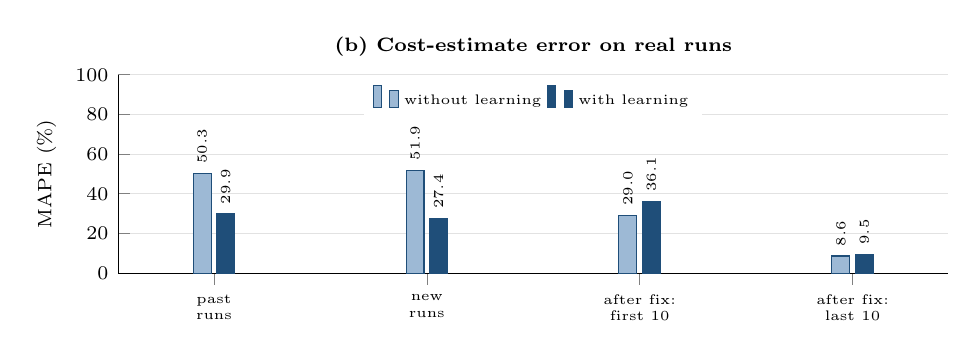
\begin{tikzpicture}
\begin{axis}[small chart, ybar, bar width=6.5pt, ymin=0, ymax=100,
  title={(b) Cost-estimate error on real runs},
  symbolic x coords={History,New runs,Fix: first 10,Fix: last 10}, xtick=data,
  x tick label style={font=\tiny, align=center},
  xticklabels={{past\\runs},{new\\runs},{after fix:\\first 10},{after fix:\\last 10}},
  ylabel={MAPE (\%)},
  enlarge x limits=0.15, legend style={at={(0.5,0.98)}, anchor=north, legend columns=2, fill=white},
  value labels, nodes near coords style={font=\tiny, rotate=90, anchor=west}]
\addplot[fill=inklight, draw=ink] coordinates {(History,50.3) (New runs,51.9) (Fix: first 10,29.0) (Fix: last 10,8.6)};
\addplot[fill=ink, draw=ink] coordinates {(History,29.9) (New runs,27.4) (Fix: first 10,36.1) (Fix: last 10,9.5)};
\legend{without learning, with learning}
\end{axis}
\end{tikzpicture}
\end{minipage}
\caption{(a) The learning agent's real code on simulated runs: it converges to within 0.04 of the
true ratio in about 35 runs, but after a sudden change its rollback rule reverts three correct moves.
(b) Paired comparisons on the same real runs. After the duration fix, the old cost factor briefly hurt,
until the loop relearned it.}
\label{fig:learn}
\end{figure}

On the same real runs, learned corrections cut cost-estimate error from 50.3\% to 29.9\% on past runs
and from 51.9\% to 27.4\% on new ones (Fig.~\ref{fig:learn}b). The live batch also showed the loop
adapting to another agent. The duration fix removed an over-estimate that the cost factor had been
compensating for, so for the first ten runs the learned factor made things worse (36.1\% against
29.0\%). Over the next 20 runs the loop moved it from 0.795 to 1.106, and error came down to 9.5\%.
All nine of its reviews confirmed their change.

The rollback rule had to be fixed first. It used to count runs that were aborted before they started,
whose ``duration'' of 0.1\,s produced post-change errors of up to 68{,}094.7\% and reverted two good
updates. Simulation shows a subtler limit that remains (Fig.~\ref{fig:learn}a): after the true ratio
jumps, each correct move is judged against an error measured before the jump, looks worse, and is rolled
back. Adaptation is delayed by about 30 runs.

\subsection{What did not work}
\label{sec:lessons}

\begin{figure}[t]
\begin{minipage}[t]{0.49\linewidth}
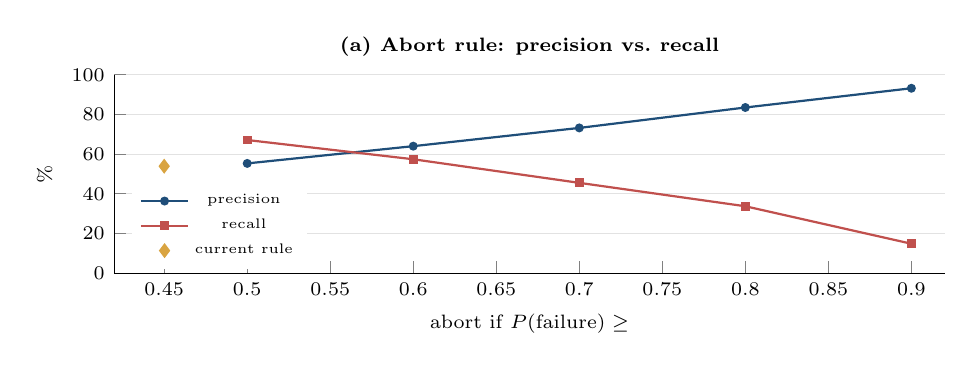
\begin{tikzpicture}
\begin{axis}[small chart, xmin=0.42, xmax=0.92, ymin=0, ymax=100,
  title={(a) Abort rule: precision vs.\ recall},
  xlabel={abort if $P(\text{failure}) \geq$}, ylabel={\%},
  legend style={at={(0.02,0.02)}, anchor=south west, fill=white}]
\addplot[ink, thick, mark=*, mark size=1.2pt] coordinates {(0.5,55.3) (0.6,64.0) (0.7,73.2) (0.8,83.5) (0.9,93.2)};
\addplot[warm, thick, mark=square*, mark size=1.2pt] coordinates {(0.5,67.1) (0.6,57.4) (0.7,45.5) (0.8,33.7) (0.9,14.8)};
\addplot[only marks, mark=diamond*, mark size=2.4pt, color=sand] coordinates {(0.45,53.9)};
\legend{precision, recall, current rule}
\end{axis}
\end{tikzpicture}
\end{minipage}\hfill
\begin{minipage}[t]{0.49\linewidth}
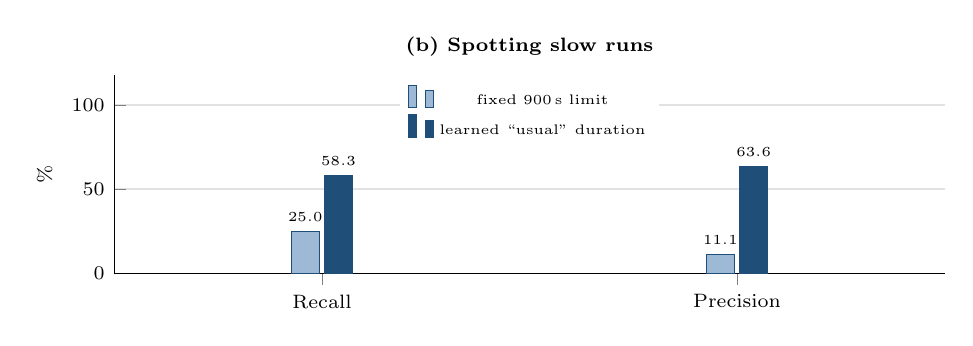
\begin{tikzpicture}
\begin{axis}[small chart, ybar, bar width=10pt, ymin=0, ymax=118,
  title={(b) Spotting slow runs},
  symbolic x coords={Recall,Precision}, xtick=data, ylabel={\%},
  enlarge x limits=0.5, legend style={at={(0.5,0.98)}, anchor=north, fill=white},
  value labels, nodes near coords style={font=\tiny}]
\addplot[fill=inklight, draw=ink] coordinates {(Recall,25.0) (Precision,11.1)};
\addplot[fill=ink, draw=ink] coordinates {(Recall,58.3) (Precision,63.6)};
\legend{fixed 900\,s limit, learned ``usual'' duration}
\end{axis}
\end{tikzpicture}
\end{minipage}
\caption{(a) The Performance Agent aborts when ``failure'' is its most likely outcome, which is right
only 53.9\% of the time on held-out data (21{,}000 runs). A 0.7 threshold trades recall for 73.2\%
precision. (b) Flagging genuinely slow runs on four pipelines of very different size (simulated, 108
runs): a per-pipeline learned baseline beats one fixed limit.}
\label{fig:gate}
\end{figure}

\paragraph{An abort rule that cries wolf.} The Performance Agent stops a run when ``failure'' is the most
likely of its three outcomes, even at $P \approx 0.5$. On held-out data that rule is right only 53.9\% of
the time (Fig.~\ref{fig:gate}a). Live, it stopped plans that then completed correctly, once when the same
stages were regrouped and once when the gate let the same plan through. A threshold of 0.7 would cut false
aborts by 72\%.

\paragraph{Completed is not correct.} Four runs finished, passed every post-run check, and were wrong. The
model had written one container name twice; the repair layer renamed the duplicate but remapped references
by name, so one stage read and wrote the same container, and the aggregation counted raw and filtered rows
together. Nothing flagged it except our output comparison. We reproduced the bug offline; the fix is to
de-duplicate by position and to add a gate rule that no stage may read its own output.

\paragraph{Playing it safe can mean doing nothing.} The Cost Agent only applies a cheaper configuration if
it can show the run will stay within a learned deadline. In 20 live runs it never could, so it never made a
run worse, and never saved a cent either.

% ===========================================================================
\section{Discussion and Limitations}

One pattern runs through the results: the learned components are good at proposing and bad at deciding.
Fine-tuning gives the planner its understanding, but repair makes the plans run; the gate, not the model,
keeps bad plans out of the cloud; and learned corrections help only behind evidence gates and rollback. The
one place a learned component decided alone, the abort rule, it was wrong almost half the time.

The evidence has limits. Live runs used one student subscription, files up to 25.5\,MB, at most three stages
and two to four repeats per configuration. The sizing, runtime and cost models are trained mostly on synthetic
data, calibrated to real telemetry where we had it, and ``actual cost'' is our cost formula at the measured
runtime, not an Azure invoice. The planner was tested on 24 requests scored by fixed patterns, which undercount
correct plans written in other styles. We count the artefacts a person would otherwise write, but we have not
yet timed people doing it.

% ===========================================================================
\section{Conclusion}

A small model that runs on a laptop, wrapped in deterministic repair and checked by gates, turned plain-English
requests into correct cloud pipelines more reliably than a model seventeen times its size, and a guarded learning
loop kept its forecasts honest on real runs. The failures taught us as much: learned gates need calibrated
thresholds, and a pipeline that completes has not necessarily done what was asked. Next, we will time engineers
on the same tasks, fix the two bugs described here, and build output checks into every run.

\subsubsection*{Disclosure of Interests.}
The authors have no competing interests to declare that are relevant to the content of this article.

% ===========================================================================
\begin{thebibliography}{99}

\bibitem{autonomic}
Kephart, J.O., Chess, D.M.: The vision of autonomic computing. Computer \textbf{36}(1), 41--50 (2003)

\bibitem{lora}
Hu, E.J., Shen, Y., Wallis, P., Allen-Zhu, Z., Li, Y., Wang, S., Wang, L., Chen, W.: LoRA: Low-rank adaptation of large language models. In: International Conference on Learning Representations (2022)

\bibitem{qlora}
Dettmers, T., Pagnoni, A., Holtzman, A., Zettlemoyer, L.: QLoRA: Efficient finetuning of quantized LLMs. In: Advances in Neural Information Processing Systems, vol.~36 (2023)

\bibitem{qwen25}
Qwen Team: Qwen2.5 technical report. arXiv preprint arXiv:2412.15115 (2024)

\bibitem{react}
Yao, S., Zhao, J., Yu, D., Du, N., Shafran, I., Narasimhan, K., Cao, Y.: ReAct: Synergizing reasoning and acting in language models. In: International Conference on Learning Representations (2023)

\bibitem{reflexion}
Shinn, N., Cassano, F., Gopinath, A., Narasimhan, K., Yao, S.: Reflexion: Language agents with verbal reinforcement learning. In: Advances in Neural Information Processing Systems, vol.~36 (2023)

\bibitem{selfrefine}
Madaan, A., Tandon, N., Gupta, P., et al.: Self-Refine: Iterative refinement with self-feedback. In: Advances in Neural Information Processing Systems, vol.~36 (2023)

\bibitem{selfcorrect}
Huang, J., Chen, X., Mishra, S., Zheng, H.S., Yu, A.W., Song, X., Zhou, D.: Large language models cannot self-correct reasoning yet. In: International Conference on Learning Representations (2024)

\bibitem{autogen}
Wu, Q., Bansal, G., Zhang, J., et al.: AutoGen: Enabling next-gen LLM applications via multi-agent conversation. arXiv preprint arXiv:2308.08155 (2023)

\bibitem{metagpt}
Hong, S., Zhuge, M., Chen, J., et al.: MetaGPT: Meta programming for a multi-agent collaborative framework. In: International Conference on Learning Representations (2024)

\bibitem{spider}
Yu, T., Zhang, R., Yang, K., et al.: Spider: A large-scale human-labeled dataset for complex and cross-domain semantic parsing and text-to-SQL task. In: Proceedings of EMNLP, pp. 3911--3921 (2018)

\bibitem{rajkumar}
Rajkumar, N., Li, R., Bahdanau, D.: Evaluating the text-to-SQL capabilities of large language models. arXiv preprint arXiv:2204.00498 (2022)

\bibitem{ottertune}
Van Aken, D., Pavlo, A., Gordon, G.J., Zhang, B.: Automatic database management system tuning through large-scale machine learning. In: Proceedings of SIGMOD, pp. 1009--1024 (2017)

\end{thebibliography}

\end{document}
